\subsection{Рынок Интернета вещей в Беларуси}
\label{sec:subject:belarus}

В 2017 году мобильный оператор velcom получил разрешение на коммерческий запуск первой в Беларуси узкополосной сети NB-IoT, предназначенной для «интернета вещей». Государственная комиссия по радиочастотам (ГКРЧ) предоставила velcom возможность использовать часть ранее выделенного компании частотного диапазона.

Специалисты называют новую технологию революционной. Беларусь станет одной из первых стран в Европе, которая запустит сеть NB-IoT (Narrow Band Internet of Things). В ближайшем будущем она может найти применение в решении различных задач – от управления «умными» счетчиками и устройствами в доме до внедрения интеллектуальных систем городского масштаба.

ГКРЧ разрешило запустить сеть NB-IoT в диапазоне 900 МГц, который сейчас используется в основном для стандарта GSM. Для «интернета вещей» velcom задействует узкую полосу частот в 200 кГц, что не повлияет на работу действующих сетей.

Стандарт NB-IoT до 30 раз превосходит используемые сейчас технологии M2M-связи по уровню проникновения сигнала. В частности, им будут покрыты труднодоступные места, в том числе подвалы, низины и здания с толстыми стенами и перекрытиями. Новый стандарт также отличают широкая область применения, экономичность и энергоэффективность \cite{iot_belarus_velcom}.

В 2018 году российская компания \enquote{МТС} также получила разрешение от ГКРЧ на создание сети NB-IoT. Для создания новых продуктов доступны все частоты в диапазоне 900 МГц, предоставленные в соответствии с решением ГКРЧ.

МТС в своей сети продемонстрировал возможности NB-IoT впервые на выставке \enquote{ТИБО-2017} совместно с компанией Huawei: была развернута тестовая зона для создания новых продуктов и сервисов. Посетители убедились в достоинствах технологии на примере конкретных продуктов: сельскохозяйственной метеостанции, трекеров для детей и домашних животных, а также "умного" замка для пунктов проката велосипедов.

В мае 2019 года МТС провела тест международного роуминга в сети стандарта Narrowband IoT (NB-IoT).

Тест прошел успешно и подтвердил возможность бесперебойной работы и непрерывного обслуживания устройств NB-IoT в гостевой сети, сообщили в МТС. Теперь российская компания готова к полноценному запуску международного роуминга NB-IoT с другими операторами.

~
\begin{figure}[H]
\centering
	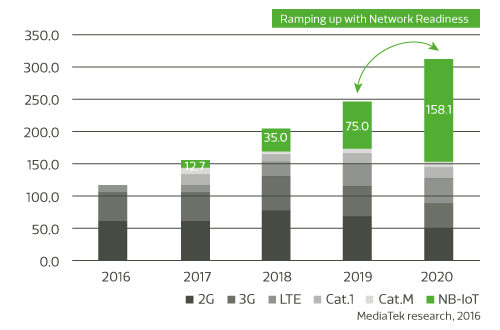
\includegraphics[scale=0.8]{figures/nbiotExample.png}
	\caption{Прогноз на распределение использования видов сотовой связи}
	\label{fig:subject:belarus:nbiot}
\end{figure}

Прогнозы таковы: в недалеком будущем большинство окружающих нас на работе и в быту вещей — от компьютера и смартфона до холодильника и фрезерного станка — будут связаны с интернетом и обмениваться с централизованным сервером или друг с другом информацией. Причем если к 2021 году количество обычных гаджетов вроде планшетов и умных телефонов увеличится до 8,7 млрд, то число IoT–устройств превысит 18 млрд. Свою пользу они будут доказывать в самых разных областях — от банального заказа холодильником недостающей еды в интернет–магазине (что фантастические фильмы предсказывали еще десятилетия назад) до полной автоматизации многих производств. Иначе говоря, условный робот–ремонтник сможет эффективно обслуживать информатизированный станок благодаря каналу связи между ними. Впрочем, заглядывать за горизонт событий совсем не обязательно: уже сегодня, допустим, БелАЗ использует IoT–концепцию и устанавливает датчики на свои большегрузы, чтобы в реальном времени отслеживать износ деталей и прогнозировать грядущий ремонт и закупку нужных запчастей \cite{iot_belarus_prog}.